

\title[Natural Phenomena as Metaphors for Visualization of Trend Data in Interactive SW Maps]%
	  {Natural Phenomena as Metaphors for Visualization of\\Trend Data in Interactive Software Maps}

\author[H. W\"{u}rfel, M. Trapp, D. Limberger, and J. D\"{o}llner]
{H. W\"{u}rfel, M. Trapp, D. Limberger, and J. D\"{o}llner
	\\
	Computer Graphics Systems Group, Hasso Plattner Institute, University of Potsdam, Germany}

\graphicspath{{figures/}}

\hyphenation{op-tical net-works semi-conduc-tor bundle-view tree-map}

% unify abbreviations
\newcommand*{\fig}[1]{Figure #1}
\newcommand*{\tab}[1]{Table #1}

\newcommand*{\eg}{{e.g.},~}
\newcommand*{\Eg}{{E.g.},~}
\newcommand*{\ie}{{i.e.},~}
\newcommand*{\ia}{{i.a.},~}
\newcommand*{\etal}{{et~al.}~}
\newcommand*{\Wrt}{{With respect to}~} %W.r.t.
\newcommand*{\wrt}{{with respect to}~} %w.r.t.

\renewcommand*{\sectionautorefname}{Section}
\renewcommand*{\subsectionautorefname}{Section}

\usepackage{wrapfig}

\usepackage{csquotes}

\usepackage{microtype}
\usepackage{amsmath}
\usepackage{amsfonts}

\usepackage{booktabs}



\begin{document}

\teaser{
	\centering
	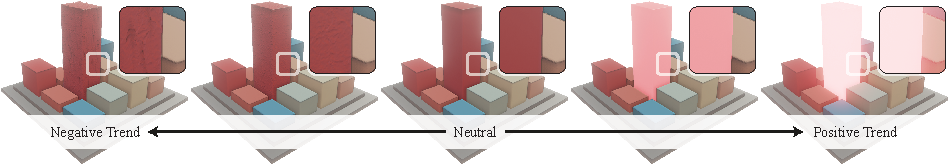
\includegraphics[width=\linewidth]{teaser}
	\label{fig:teaser} 
	\bigskip %
}

\maketitle


\begin{abstract}

Software maps are a commonly used tool for code quality monitoring in software-development projects and decision making processes. 
While providing an important visualization technique for the hierarchical system structure of a single software revision, they lack capabilities with respect to the visualization of changes over multiple revisions. 
This paper presents a novel technique for visualizing the evolution of the software system structure based on software metric trends. 
These trend maps extend software maps by using real-time rendering techniques for natural phenomena yielding additional visual variables that can be effectively used for the communication of changes. 
Therefore, trend data is automatically computed by hierarchically aggregating software metrics. 
We demonstrate and discuss the presented technique using two real world data sets of complex software systems.

\begin{classification} % according to http://www.acm.org/class/1998/
	\CCScat{Software Engineering}{D.2.2}{Design Tools and Techniques}{Computer-aided software engineering (CASE)}
	\CCScat{Software Engineering}{D.2.7}{Distribution, Maintenance, and Enhancement}{Documentation}
	\CCScat{Computer Graphics}{I.3.7}{Three-Dimensional Graphics and Realism }{Color, shading, shadowing, and texture}
\end{classification}

\end{abstract}


\section{Introduction}
\label{sec:introduction}

\noindent 
Almost every software system is subject to constant change due to evolving technology and user requirements. 
Its continuous development is largely driven by corrective, adaptive, perfective as well as preventive maintenance \cite{Lientz1980}.
The responsible development teams undergo changes as well and developers not involved in the previous development process are required to spent a considerable amount of their time understanding the system under maintenance. 
Furthermore, creating a mental model of a software is difficult, as it is virtual and intangible \cite{Knight2000}, thus, making it hard to communicate the structure and behavior of the system to decision makers. 
Visualization tools can provide communication artifacts such as software maps that assist software engineering and maintenance, \eg by allowing for actionable insights.

In recent years software maps were established to communicate static, dynamic, and evolutionary information of software systems as well as their software development processes by means of information visualization. 
The application of 2D or 3D map-oriented techniques constitute a fundamental approach in software visualization, software analytics, and software diagnosis.
Its primary applications include risk analysis for and monitoring of code quality, team activity, or software development progress \cite{Bohnet2011}.

\paragraph*{Evolution of Software Systems}
\noindent
The evolution of a software system can be tracked by, \eg revision control systems, making it possible to analyze changes over revision ranges by sampling revisions over time.
This information can be used for example to retrace, whether a design decision (\eg an architectural refactoring) resulted in an expected change that manifests itself in an improvement of respective \emph{software metrics}.
Existing approaches either use transition animations between multiple revisions to depict the evolution process or they convey a progress within a single static image:
Transition animations have the advantage of keeping the established metric mappings but do not scale for large software system or revision ranges with much change information to be displayed at once.
Conveying the characteristics of an evolution process within a static image does not suffer from this problem but existing approaches sacrifice at least one attribute mapping to encode an evolution measure.

\paragraph*{Metaphors for Trend Visualization}
\noindent
To overcome those shortcomings, a software map which uses natural phenomena as metaphors to visualize software metric trends within a static representation (\emph{trend map}) is used. 
In this paper, a static representation of the trend map denotes a visualization artifact that exhibits no transition animation with a revision range, but it can be explored using 3D interaction metaphors \cite{Jankowski2013}.
It combines the visualization of the static system structure with evolutionary information by augmenting interactive software maps with additional visual variables represented by natural phenomena (\eg fire, rain) or material properties (\eg rust, shininess, glow). 
Thereby, the visual variables that are used to depict the properties of the static system structure by mapping software metrics to color, area, and height can be maintained. 
Furthermore, the automatic computation of trends in metrics (\emph{metrics trends}) enables forecasting their future course, \eg increase, decrease, and stagnation. 
With the support of specific software metrics trends, decision makers can initiate preventive maintenance actions.

\begin{figure}[tbp]
	\centering
	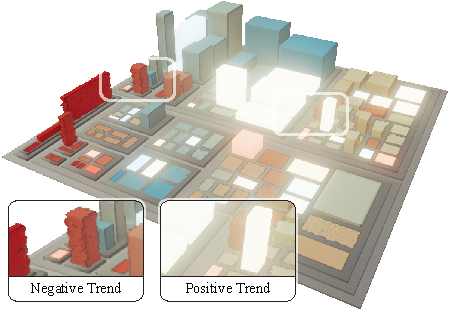
\includegraphics[width=\linewidth]{trendmap}
	\caption{
		This example depicts the trend of a system's test-coverage: 
		Area comprises lines-of-code, height relates to source code complexity, and color indicates test-coverage (red for lower and blue for higher coverage).
		Glowing items depict a positive trend, while a rough surface symbolizes a decrease in test-coverage during a specific time interval.}
	\label{fig:trendmap}
\end{figure}

When faced with unfamiliar concepts, our cognitive system searches for the best mapping between the unknown concept and existing knowledge of other domains \cite{Zhang2008}.
Software maps use a virtual city metaphor yielding a familiar 2.5D reference geometry. 
In this context, the application of natural phenomena as metaphors seems promising, since it can be assumed that they closely match to virtual 3D environments:
At best, their semantics are intuitively decoded making an additional legend non-obligatory. 
Examples of natural phenomena are objects aging in terms of their associated materials or degeneration within their environment (overgrown by grass, silted, gathering dust), changing in radiant emittance, as well as being exposed to natural forces such as fire, rain, wind, or sunshine (\autoref{fig:trendmap}).

\paragraph*{Challenges \& Contributions}
\noindent
A main challenge is the identification of natural phenomena that are suitable to effectively communicate trend data.
For it, metric values have to be mapped to parameters of respective rendering techniques in a comprehensive way. 
Furthermore, to extend their application to hierarchical structuring elements (\eg software modules) instead of individual leaf items only, hierarchical metric value aggregation is required. 
All in all, the challenges for an interactive visualization of trend data using natural phenomena as metaphors within software maps comprise
(1) a concept for mapping natural phenomena to software map items, 
(2) the aggregation of software metric values within revision ranges, 
(3) the metrics based parametrization of rendering techniques, and 
(4) rendering within real-time constraints.

With respect to these challenges, this paper contributes:
\begin{enumerate}

	\item A novel concept for the visualization of trend data within interactive software maps using natural phenomena.

	\item A technique for hierarchical aggregation of software system information and metrics automatically extracted from, \eg, revision control systems as well as a respective mapping to parametrize the real-time rendering techniques used for synthesis of natural phenomena.

	\item A prototypical implementation using the Unreal Engine 4 \cite{UnrealEngine4} capable of handling actual software system data.
	
\end{enumerate}

\noindent 
The remainder of this paper is structured as follows.
Related work \wrt interactive software visualization is reviewed in \autoref{sec:related}.
\autoref{sec:metaphors} presents a concept for trend visualization using item-based and context-based metaphors and \autoref{sec:design_and_parametrization} describes our hierarchical metric aggregation.
A prototype is briefly described in \autoref{sec:implementation} and demonstrated using actual software system data presented and discussed in \autoref{sec:results}. 
Finally, \autoref{sec:conclusions} concludes this work.


\section{Related Work}
\label{sec:related}
\noindent 
Related work comprises the fields of 2.5D software maps and metaphor-based visualization of software system evolution.

\paragraph*{Interactive Software Maps}

Treemaps are commonly used to visualize hierarchical datasets. 
The original space-filling algorithm introduced by \cite{Shneiderman1992} slices parent nodes recursively by their child nodes' properties, alternating in horizontal and vertical direction. 
Due to undesirable aspect ratios produced by this slice and dice algorithm, Bruls \etal as well as Bederson and Shneiderman proposed squarified treemaps \cite{Bruls1999} and strip treemaps \cite{Bederson2002}. 
Furthermore, while preserving the visualization of the hierarchy, Fekete and Plaisant added visual attributes, such as color and size, to treemap items \cite{Fekete2002}. 
The first 2.5D treemap was described in the \emph{Step Tree} approach presented by Bladh \etal \cite{Bladh2004}. 
The geometric representation of sub-directories is stacked on top of their parent directories. 
This extension to the third dimension enables metaphor-based visualizations as shown in \emph{Information Pyramids} \cite{Andrews1997} and \emph{Code City} \cite{Wettel2008}, a city metaphor for 3D treemaps in which the height of the treemap's cuboids is used to map an additional software system metric. 
Similar to actual cities, these code cities are partitioned into several districts, including downtown areas and suburbs.
Referenced as \emph{software maps}, the city metaphor was adopted and extended by several other publications \cite{Liggesmeyer2009,Bohnet2011}.
Bohnet and D{\"o}llner describe the usage of software maps as a decision-making tool.
Recently, a comparative performance evaluation of rendering techniques for 2.5D treemaps was presented \cite{Trapp2013}.
With it, a deferred shape-generation algorithm outperforming existing approaches is presented.
The basic idea is to generate and render an attributed point-cloud and to expand the points to cuboids on the GPU.

\paragraph*{Visualization of Software Evolution}

The visualization of software evolution implies an additional time dimension.
Most techniques visualize the change process by animating the transition phase between two software revisions.
The \emph{VERSO visualization tool} \cite{Langelier2008} uses linear interpolation of color, height, and twist between two revisions. 
Another approach uses an Evolution Storyboard consisting of an ordered sequence of animated panels showing the structural changes during a time period \cite{Beyer2006}.
In contrast to animation, the Evolution Matrix approach displays the entire evolution of the software system in a single image \cite{Lanza2001}. 
Rectangles are used to map the number of methods to width and the number of attributes to height. 
Each revision is visualized next to its consecutive revision in a separate column.

\paragraph*{Metaphors in Software Visualization}

Besides the city metaphor, other metaphors for software system visualization were proposed. 
Balzer \etal presented a software landscape metaphor \cite{Balzer2004} using landscape-like distributions of three-dimensional objects on a 2D reference plane. 
Depending relationships between subsystems are visualized using a hierarchical network. 
Further, Graham \etal proposed a solar-system metaphor \cite{Graham2004} for object-oriented software metrics.
Planets represent classes, orbits depict the inheritance level within a package: planets in each orbit represent an inheritance hierarchy, while the lines-of-code of a class are mapped to the planet size. 
A thoroughly written survey of visualization techniques for static and evolutionary information of software systems is presented by Caserta and Zendra \cite{Caserta2011}.
Holten \etal presented a 2D treemap visualization of software metrics using the surface structure of treemap elements by applying texture- and bump mapping to them \cite{Holten2005}. 
Their approach is based on the fact that the human visual system can rapidly process visual cues such as shading and textures \cite{Enns1990,Healey1998,Healey1999}.
Panas \etal use a realistic city metaphor to map code quality metrics to building textures \cite{Caserta2011}. 
Furthermore, they proposed visual effects such as fire and bolts to communicate hot spot information in code execution and frequent component modifications \cite{Panas2003}.
However, neither an implementation nor an evaluation of such visual mappings are provided.
An empirical study by Borgo \etal suggests that visual embellishments aid memorization performance in both accuracy and response time, though it might have a negative impact on speed of visual search \cite{Borgo2012}.
It further proves that visual embellishments aid concept grasping.



\section{Natural Phenomena as Metaphors for Software Maps}
\label{sec:metaphors}
\noindent
The proposed concept of trend maps is a metaphorical extension to existing interactive software maps. 
However, there are various definitions of metaphors in multiple science disciplines. 
Hereinafter, a metaphor consists of a \emph{target domain}, \emph{target item}, \emph{source domain}, \emph{source item}, and \emph{matching part} \cite{Zhang2008}.
The source item (\eg weathering effect) from a well-known source domain (natural phenomena) is mapped to target items (cuboids representing software entities) of the target domain (software maps).
The target domain is relatively unknown and the match will never be perfect.
However, the larger the matching part the better the metaphor works.

\begin{figure*}[t]
	\centering
	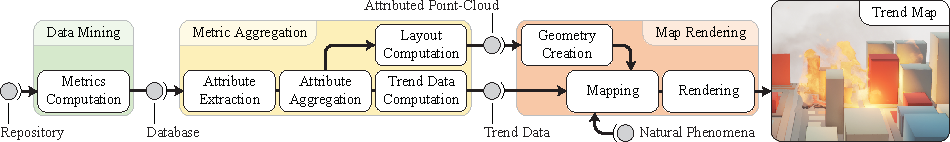
\includegraphics[width=1.0\textwidth]{pipeline}
	\caption{Schematic overview (data and control flow) of our trend map pipeline comprising three conceptual stages.}
	\label{fig:pipeline}
\end{figure*}

\subsection{Preliminaries and Assumptions}
\noindent
For the usage of natural phenomena we assume an appropriate match. 
This assumption is made due to our prior experience in assessing the semantics of natural phenomena. 
Furthermore, it is based on human usage of linguistic metaphors in idioms concerning natural phenomena such as \enquote{to go up in flames} and \enquote{grow grass upon}.
\Wrt the application and design of natural phenomena, we further assume that their image-synthesis can be performed in real-time to facilitate an interactive system.
Therefore, this paper focuses on hardware-accelerated rasterization for real-time rendering \cite{Akenine2008}.

\subsection{Conceptual Overview}
\noindent
Our approach is structured as pipeline comprising data mining, metrics aggregation, and trend map rendering (\autoref{fig:pipeline}).

\paragraph*{Data Mining}
\noindent
At first, software metrics are computed on a per-item basis. 
Therefore, each revision of a software system is analyzed independently.
The resulting artifact is a \emph{database} encoding a revision tree per revision.
This step is performed once for a given repository and allows for successive updates if new revisions have to be considered.

\paragraph*{Metric Aggregation}
\noindent
In this stage, a revision range $R = [n,\;m]$ with $n,m \in \mathbb{N}, n < m$ is specified by the user and used to compute the trend data later.
The user also selects the metrics of which he wants to observe trends.
The trend data of every treemap item is defined as a time series of metric data points over the revision range: 
For example, items that already existed at the start revision $n$ and outlast the end revision $m$, consist of a time series with $m-n+1$ data points.
Trend data is then aggregated with respect to particular parent items of the hierarchy. 
Subsequently, a treemap layout is computed and encoded as \emph{attributed point-cloud} for efficient rendering in the next stage. 
Simultaneously, the \emph{trend data} is computed by analyzing the time series for all treemap items.

\paragraph*{Map Rendering}
\noindent
The rectangular treemap geometry is created based on the attributed point cloud. 
Trends are mapped to the parametrization of natural phenomena (\autoref{sec:design_and_parametrization}).
Depending on the degree of change, five discrete levels are depicted in one trend map to facilitate visual distinction: strong increase, moderate increase, stagnation, moderate decrease, and strong decrease.
Up to two distinct effects can be specified by the user, one for negative and one for a positive trend. 
The effects are parametrized according to the computed trend and combined with the static system structure encoded in the attributed point-cloud.
The latter is used for final image synthesis (\autoref{sec:implementation}).

\section{Design and Parametrization of Natural Phenomena}
\label{sec:design_and_parametrization}
\noindent
Before focusing on suitable metaphors and their automatic parametrization, this section describes the design space of natural phenomena and how these can be mapped to software maps for effective visual communication. 
Considering 2.5D treemaps as reference geometry \cite{Duebel2014}, a differentiation between \emph{item-based} and \emph{context-based} metaphors, can be made \wrt the \emph{design elements}:
\begin{description}
	
	\item[Item-based metaphors] Modifying the visualization of a single treemap item by changing its surface appearance using additional or altered materials,
	
	\item[Context-based metaphors] Modifying a group of treemap items or modifying their surrounding context (3D space) of the visualization elements affected.
	
\end{description}

\subsection{Item-based Metaphors}
\noindent 
The surface properties of a treemap cuboid define a material that determines how light interacts with them and hence how it is perceived.
To find suitable metaphors to communicate the change of an object state over time we pair contrary phenomena (\autoref{fig:item-based-metaphors}). 
We identified the roughness of a surface to be a suitable metaphor to visualize \enquote{how neat} a component implementation is:
A negative trend is depicted by a high surface roughness, optionally amplified by texture based (displacment mapping) as well as geometry based (tessellation) displacement (\emph{rough}). 
In contrast thereto, a positive trend is depicted using a low surface roughness in combination with a
high specular reflection property, resulting in a shiny and clean cuboid (\emph{shiny}).
Concerning the evolution of test coverage of individual items, corrosion is a suitable metaphor.
Thereby, high degree of corrosion relates to decreasing test coverage (\emph{rusty}).
Due to the fact that no corrosion would result in the neutral state (which results from the applied color mapping), a high radiant emittance (glow) is used to effectively communicate a positive trend in test coverage (\emph{glowing}). 
\begin{figure}[b]
	\centering
	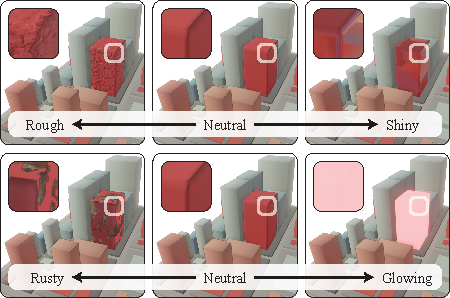
\includegraphics[width=1.0\linewidth]{item-based-metaphors}
	\caption{Two examples for item-based metaphors covering the transition between negative and positive object states.}
	\label{fig:item-based-metaphors}
\end{figure}

\subsection{Context-based Metaphors}
\noindent
\begin{figure*}[t]
	\centering
	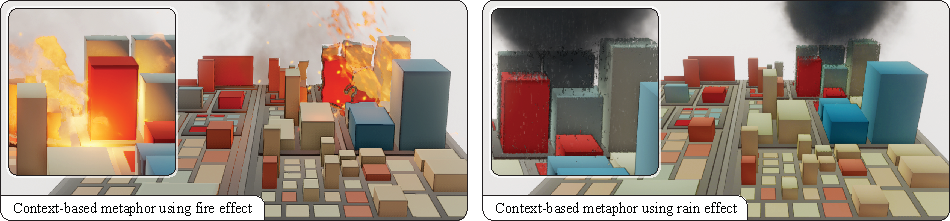
\includegraphics[width=1.0\textwidth]{context-based-metaphors}
	\caption{Context-based metaphors, automatically assigned to development hot spots (\eg strong decrease or stagnation).}
	\label{fig:context-based-metaphors}
\end{figure*}
Context-based metaphors are either natural phenomena or effects that affect the area surrounding treemap items or a group of adjacent items. 
In order to parametrize such effects properly, context-based metaphors require information about the hierarchical aggregation of software metrics to determine trends for parent items. 
Particle systems are mainly used to visually communicate hot spots (or regions-of-interest) in source code, \eg so-called \enquote{code smells}. 
Therefore, we use a fire effect or rain (\autoref{fig:context-based-metaphors}) to indicate negative trends.

\subsection{Trend-based Parametrization}
\noindent
To fully automate the trend-based parametrization, each effect contains a self description comprising all of its parameters. 
A single \emph{parameter description} consists of the \emph{parameter type} (\ie vector, scalar, and color), the value range $[i_{\mathrm{min}},\;i_{\mathrm{max}}]$ of the parameter $v$, a \emph{default value} and a boolean value that determines whether to \emph{inverse} the mapping or not (\eg a positive trend is mapped to a roughness of zero).
The parametrization is performed by mapping the trend $v$ from an input trend value range $[i_{\mathrm{min}},\; i_{\mathrm{max}}]$ to an output parameter value range $[j_{\mathrm{min}},\;j_{\mathrm{max}}]$ by 
$  v_{\mathrm{mapped}} = (v - i_{\mathrm{min}})\frac{j_{\mathrm{max}} - j_{\mathrm{min}}}{i_{\mathrm{max}} - i_{\mathrm{min}}} + j_{\mathrm{min}}$.
Every effect defines parameter sub-ranges that discretize the mapped parameter value $v_{\mathrm{mapped}}$ to the five categories: \emph{strong increase}, \emph{increase}, \emph{stagnation}, \emph{decrease}, or \emph{strong decrease}.

\subsection{Hierarchical Aggregation of Software Metrics}
\noindent
Similar to software maps, the hierarchical structure of trend map mirrors the directory tree of the current revision chosen from a code repository. 
To determine software metric trends for individual (\ie files) as well as groups of items (\eg packages), trend data is aggregated bottom-up within the hierarchy in a specified revision range.
Post-order and reversed level-order traversals are suitable for this task. 
Therefore, a node in a revision range tree holds a bucket $k$ for each revision within the revision range. 
The respective metric value  $x_k$ contained in the bucket is computed using \emph{weighted average}.
Empty buckets represent items that are not present in a specific revision. 
The weights $w_k$ are determined by counting the leaf nodes in the sub-tree where the node for which we want to aggregate the metric values is the root node.


\section{Implementation Overview}
\label{sec:implementation}
\noindent
In contrast to previous work in the field of software visualization, our approach is based on utilizing the rendering capabilities of modern GPUs for image synthesis of 2.5D treemaps that are augmented with complex surface materials and particle systems in real-time (\autoref{fig:implementation-ue4}).

\subsection{Rendering Engine Integration}
\noindent
We have chosen to evaluate the Unreal Engine 4 (\emph{UE4}) for our prototypical implementation since it lets us rapidly prototype materials and particle systems for our purposes. 
At the date of writing, Unreal Engine 4.8 is the latest iteration of the game engine created by Epic Games Inc. 
It offers libraries and tools as well as the engine's source code to develop graphics applications.
Game development in C++ with UE4 works by implementing a shared library (game module) which is loaded by the engine at runtime. 
To change or extend the engine functionality there are two options: source code modifications and plugins. 
We have integrated our own software visualization library using plugins and instead of our own renderer, we use the Unreal renderer. 
The game module uses the plugin to visualize the trend map and implements a basic navigation and graphical user interface to interact with it.

\subsection{Surface Materials for Item-based Metaphors}
\noindent
Shaders for rendering surfaces are denoted as \emph{surface materials} in UE4. 
Usually, they are developed using a visual interface in a material editor based on creating a directed acyclic graph (\emph{DAG}) of operations.
Internally, these DAGs are compiled to shader code. 
UE4 implements a physically-based shading model with a small set of intuitive parameters (base color, metallic, specular, roughness, emissive color). 
\setlength{\columnsep}{\marginparsep}
\setlength{\intextsep}{-0.5\marginparsep}

\noindent
\begin{wrapfigure}{l}{0.5in}
	
\includegraphics[width=0.5in]{material-rust}
\end{wrapfigure}
\textbf{Rust} is modeled using multi-texturing: The combination of color and texture (rust distribution) is controlled using Perlin noise with two octaves.

\noindent
\textbf{Radiant emittance} is modeled by setting the base color as well as the emissive color multiplied by an emissive strength to the vertex color of the respective cuboid. 

\noindent
\begin{wrapfigure}{l}{0.5in}
	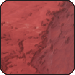
\includegraphics[width=0.5in]{material-roughness}
	\vspace{0.1in}
\end{wrapfigure}
\textbf{Roughness} is implemented using a combination of geometry tessellation, normal mapping, and vertex displacement along a normal vector that represents the original surface orientation modified using a 3D noise function.

\noindent
\begin{wrapfigure}{l}{0.5in}
	
\includegraphics[width=0.5in]{material-shininess}
\end{wrapfigure}
\textbf{Shininess} is created using the metallic parameter, with a high specular value and roughness close to or equal to zero. 

\setlength{\columnsep}{\marginparsep}
\setlength{\intextsep}{\marginparsep}

\begin{figure}[b]
	\centering
	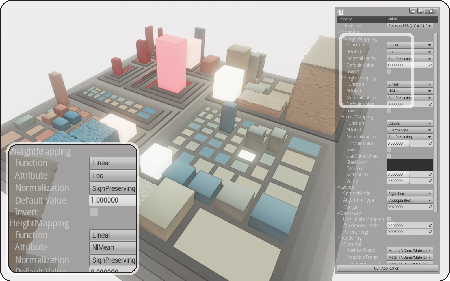
\includegraphics[width=1.0\linewidth]{implementation-ue4}
	\caption{Unreal editor showing a trend map during setup.}
	\label{fig:implementation-ue4}
\end{figure}

\subsection{Particle Systems for Context-based Metaphors}
\noindent
Similar to surface materials, particle systems can be configured visually in an interactive editor. 
Multiple emitters can be specified and each emitter comprises various parameters such as spawning rate, collision behavior with scene geometry, and particle color and size. 
Ideally, a particle system is instantiated inside the bounding box of its affected item group. 
Since the engine (as of this writing) does not offer the option to specify a dynamic volume for the particle systems, we work around this by spawning several particle systems inside the bounding
box.
To ensure a minimum distance between multiple systems, Poisson disk sampling is used \cite{Bridson2007}.

\subsection{Automatic Effect Parametrization}
\noindent
For item-based effects, the parametrization is based on the material system.
The material parameters are mirrored in a material representation in main memory.
We change material properties at runtime by querying the materials defined as negative or positive trend as well as their corresponding parameter descriptions, and finally applying a trend-dependent parametrization.
The trend is computed over a revision range by analyzing the time series using linear regression. 
By assuming that the underlying trend function is linear, the slope of the trend line can be used to discretize the trend easily into the previously used five categories. 

However, a linear regression model for time series is rarely the best choice, since 
(1) its deviation from the data is often larger at the end of the time series or 
(2) the underlying data is simply not linear. 
Our system is designed to be extensible to different trend computation models, since other prediction models might be better suited.
For an overview of statistical forecasting methods and respective application scenarios we refer to Robert F. Nau \cite{Nau2015}.

A material is also an implementation of an element-based effect. 
Context-based metaphors using surface properties are implemented top-down by propagating aggregated metric values down the hierarchy. 
Particle systems are handled in a similar manner.


\section{Results and Discussion}
\label{sec:results}
\noindent 
The results of our technique are discussed by means of application examples using real-world data sets and directions for future research are provided.
\begin{figure*}[t]
	\centering
	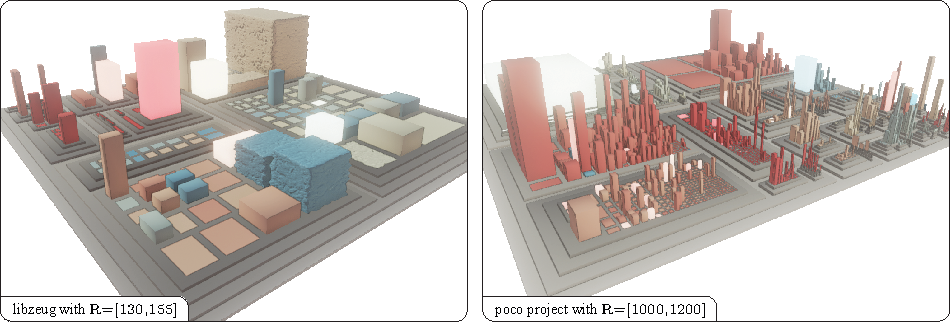
\includegraphics[width=1.0\textwidth]{results}
	\caption{
		Applications of the presented visualization technique using two real data sets using item-based natural phenomena as metaphors.
		The underlying software maps encode lines-of-code to item area, the mean nesting-level to height, and the number of file changes within the revision range to color. 
		Left: the trends of the McCabe metric is mapped into the range between a rough surface and glow. 
		Right: the inverted trend of the lines-of-code metric is mapped using the same metaphor.}
	\label{fig:results}
\end{figure*}
\Wrt to performance, the technique was tested using datasets of two software systems with different complexity, \ie different static structure components and number of revisions (\autoref{fig:results}):
\begin{table}[h]
	\centering
	\begin{tabular}{llll}
		\textbf{Data Set} & \textbf{\#Rev.} & \textbf{Rev. Range} & \textbf{max. \# Items} \\
		\midrule
		libzeug & 248 & [130,155] & 243 \\
		PocoProject & 2038 & [1000,1200] & 2635 \\
	\end{tabular}
\end{table}
\\
For each revision, the repository was downloaded, making it yet impractical for repositories containing binary files.
Gathering the revision data, computing and aggregating metric values for 72 software metrics for every revision of the master branch resulted in expensive preprocessing.
However, both projects can be rendered at interactive frame rates:
\begin{table}[h]
	\centering
	\begin{tabular}{llll}
		\textbf{Data Set} & \textbf{Metric Comp.} & \textbf{Aggr.} & \textbf{Rendering} \\
		\midrule
		libzeug     & appr. 04h & 04sec & 16ms \\
		PocoProject & appr. 48h & 17min & 43ms \\
	\end{tabular}
\end{table}

Our trend maps facilitate the depiction of metric changes over a revision range by extending software maps of a certain revision $x \in R$. 
Hence, a conceptual limitation of our approach, is that a trend map only shows trends for items which are still present at the respective revision $x$. 
A proper visualization of deleted or added system components within a software map is still subject to research.

Besides the static image approach for our trend maps, we have also tested several animated transitions for trend data of a revision range.
We tested linear interpolation and cubic interpolations using uniform, chordal, and centripetal catmull-rom splines \cite{Yuksel2009}. 
By additionally rendering these trend curves the user gets a familiar view to explore the trend data of a particular item or a group of items.
However, we found that using these trend curves to parametrize the natural phenomena during a transition animation overstrains the user's perception for complex real-world data sets, since there are too many change processes visualized simultaneously.

The presented approach can be used to facilitate overview of hot spots in software maps according to the information \enquote{seeking mantra: overview first, zoom and filter, then details-on-demand} \cite{Shneiderman1996}.
Especially effects such as glow seem to support pre-attentive processing and can be used for
highlighting purposes, but in contrast to rust or shiny effects, it alters the item's color mapping significantly and complicates the perception of shape. 
However, the perception of surface effects such as rust or corrosion depends on items' screen sizes.
Also, when depicting larger revision ranges the number of affected items and regions tend to cause cluttering and context-based metaphors (\eg fire) comprising large regions-of-interest sometimes cause occlusion. 

\paragraph*{Future Work}
We plan to focus our research on evaluation and adjustment of the visual metaphors by conducting a comprehensive user study. 
\Wrt this, research on how certain effects (\eg fire or thunderstorms) are able to emotionalize.
Furthermore, care has to be taken on how many natural phenomena implemented can be applied simultaneously and still be perceived and distinguished by users (\autoref{fig:additional-result}).
Another topic for future work can be to evaluate different forecasting methods for software metrics and directly map them to metaphors commonly used in daily weather forecasting visualizations.
To allow for natural phenomena to be used on larger data sets, level-of-detail (LoD) compliance of the presented techniques has to be evaluated, \eg for surface appearances, since fine surface details are hard to perceive if the virtual camera is far away from a region-of-interest.

\begin{figure}[b]
	\centering
	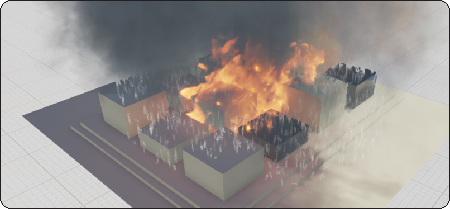
\includegraphics[width=1.0\linewidth]{additional-result}
	\caption{Superposition of multiple natural phenomena.}
	\label{fig:additional-result}
\end{figure}

\section{Conclusions}
\label{sec:conclusions}
\noindent
This paper presented \emph{trend maps}, a novel technique using natural phenomena as metaphors for visualizing the evolution of software system structures based on software metric trends.
It has been demonstrated that by analyzing the time series of software metric values and visualizing their trends using our technique, it is possible to communicate the (1) number, (2) magnitude, and (3) gradient of software metric changes. 
Based on our experiences with the prototypical implementation, natural phenomena can also be used to emotionalize the visual communication by providing memorable visualizations of the software system. 

This research was concerned with the application of natural phenomena within interactive software maps; however, the results may also be applicable to other fields in information visualization, though, caution in applying metaphors in visualization remains advisable.


\section*{Acknowledgments}
\label{sec:acknowledgments}
\noindent 
The authors would like to thank the anonymous reviewers as well as Martin R\"{o}hlig for their valuable comments. 
This work was funded by the Federal Ministry of Education and Research (BMBF), Germany, within the InnoProfile Transfer research group \enquote{4DnD-Vis} (\url{www.4dndvis.de}).

\newpage

\bibliographystyle{eg-alpha}
\bibliography{naturalmetaphors}

\end{document}
